\section{Optimization}

\sectionPage{Optimization}

\begin{frame}[fragile]{Optimization}{}
	\lstset{language=Python}
	\begin{lstlisting}[basicstyle=\tiny]
...
res = optmze.brute(compareGainCurve, bnds, full_output=True, finish=optmze.fmin)
...
res = optmze.minimize(compareGainCurve, x0, bounds=bnds, options={'disp': True, 'eps': 0.5})
...
x1 = np.array([-28.22, 5.65, 110.14, 2044.41, -33.94, 0.])
...
	\end{lstlisting}
\end{frame}

\begin{frame}[c]{Optimization: Results}{}
	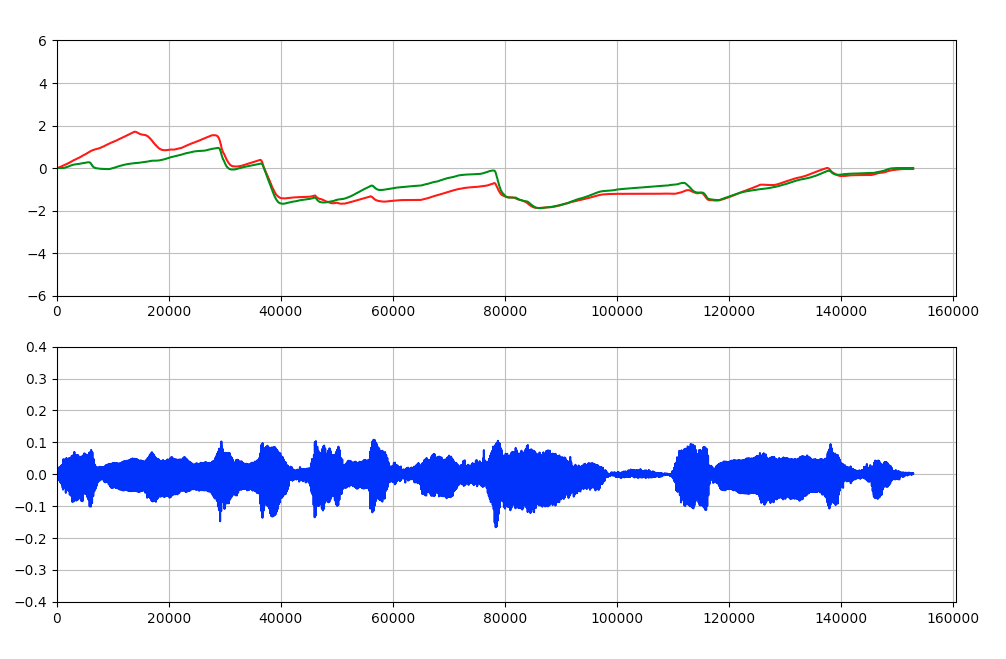
\includegraphics[scale=0.32]{images/optiG}
	\centering
\end{frame}
